\section{Platform Interface}

\subsection{Public-facing views}

The public side of the platform is designed to make the curated database accessible without forcing users into the Django admin. The homepage introduces the purpose of the project and links directly to the browser and graph views. The browser landing page then presents the main record categories available for exploration.

List pages expose the main evidence types in a structured way. Studies can be browsed at paper level, groups and comparisons can be inspected to understand study design, taxa can be explored using lineage-aware filters, and findings can be searched directly. This supports both top-down exploration, such as starting from a disease or paper, and bottom-up exploration, such as starting from a taxon.

The browser is especially important because it turns the schema into something operational for users. A good data model is not very useful if the resulting records remain buried inside raw tables. By exposing records through searchable and filterable pages, the platform makes the curated content inspectable and therefore more trustworthy.

\begin{figure}[htbp]
    \centering
    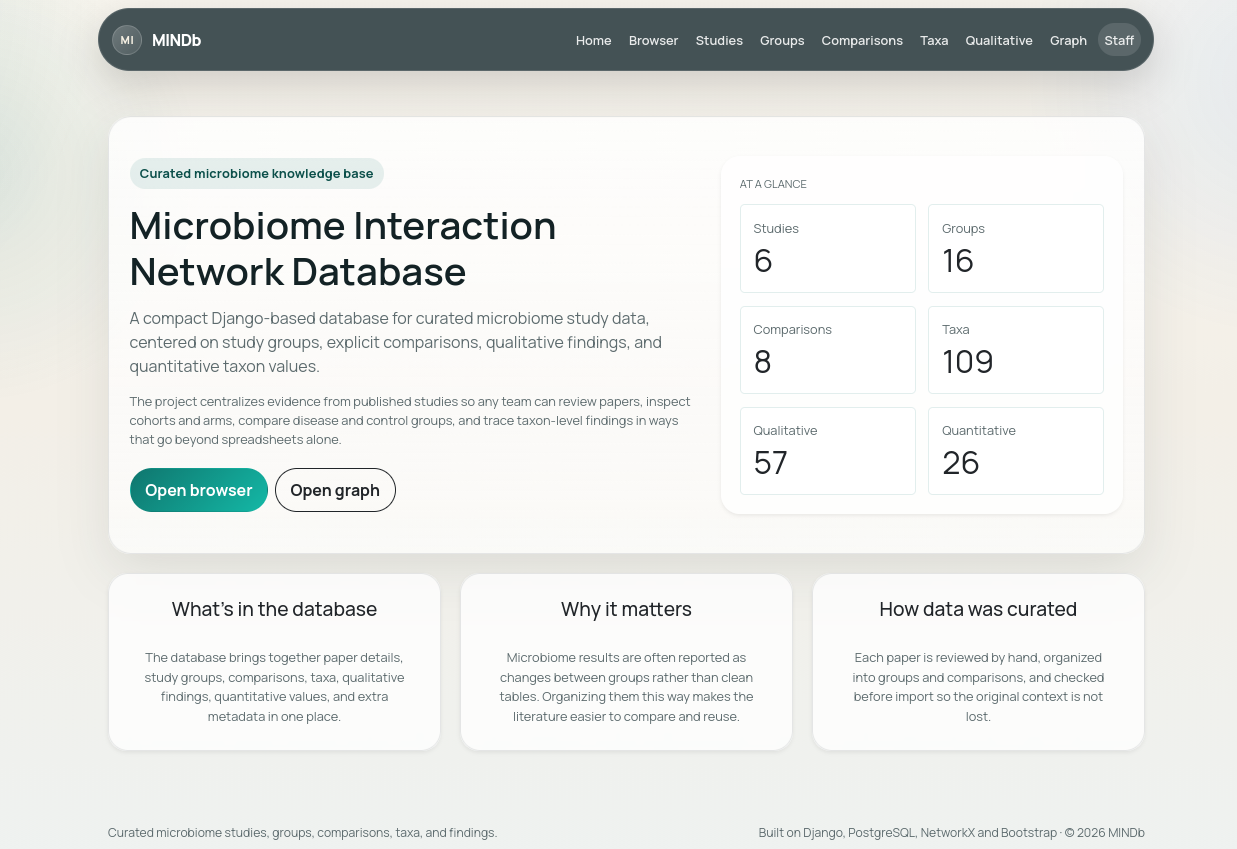
\includegraphics[width=\linewidth]{figures/mindb_homepage.png}
    \caption{Homepage of the \projectname{} platform, presenting the project purpose and linking to the browser and graph views.}
    \label{fig:homepage}
\end{figure}

\begin{figure}[htbp]
    \centering
    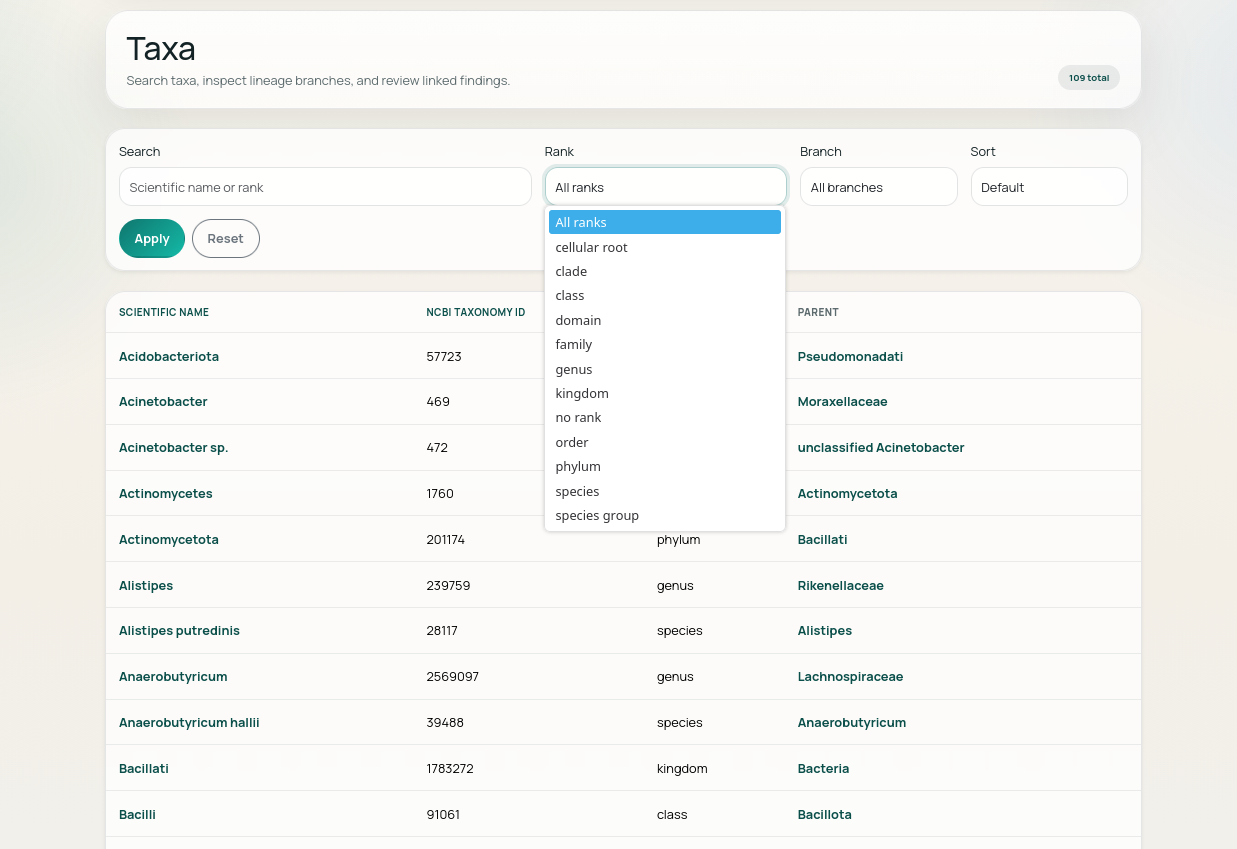
\includegraphics[width=\linewidth]{figures/mindb_browser.png}
    \caption{Example of the structured browser interface used to search, filter, sort, and inspect curated records.}
    \label{fig:browser}
\end{figure}

\subsection{Curation and administration}

The platform also includes staff-only functionality for curation and maintenance. A protected staff workspace links to import tools, the Django admin, and a generated model diagram. Through Django admin, curators can edit studies, groups, comparisons, taxa, qualitative findings, quantitative findings, metadata variables, metadata values, diversity metrics, and import batches. The admin environment also supports broader platform administration such as user management and permission-aware access control through Django's standard administrative system.

From a project perspective, this matters because literature curation is not only a viewing problem. It is also a data stewardship problem. The ability to maintain records manually, inspect schema structure, and upload new content through a validated workflow is essential to the usefulness of the platform.

The combination of manual admin editing and structured batch upload is deliberate. Some corrections are easiest to make one record at a time, especially during early prototyping or spot fixes. Other tasks, such as ingesting curated workbook content, are more efficient through batch-oriented import. Supporting both modes makes the system more realistic as a curation platform.

\begin{figure}[htbp]
    \centering
    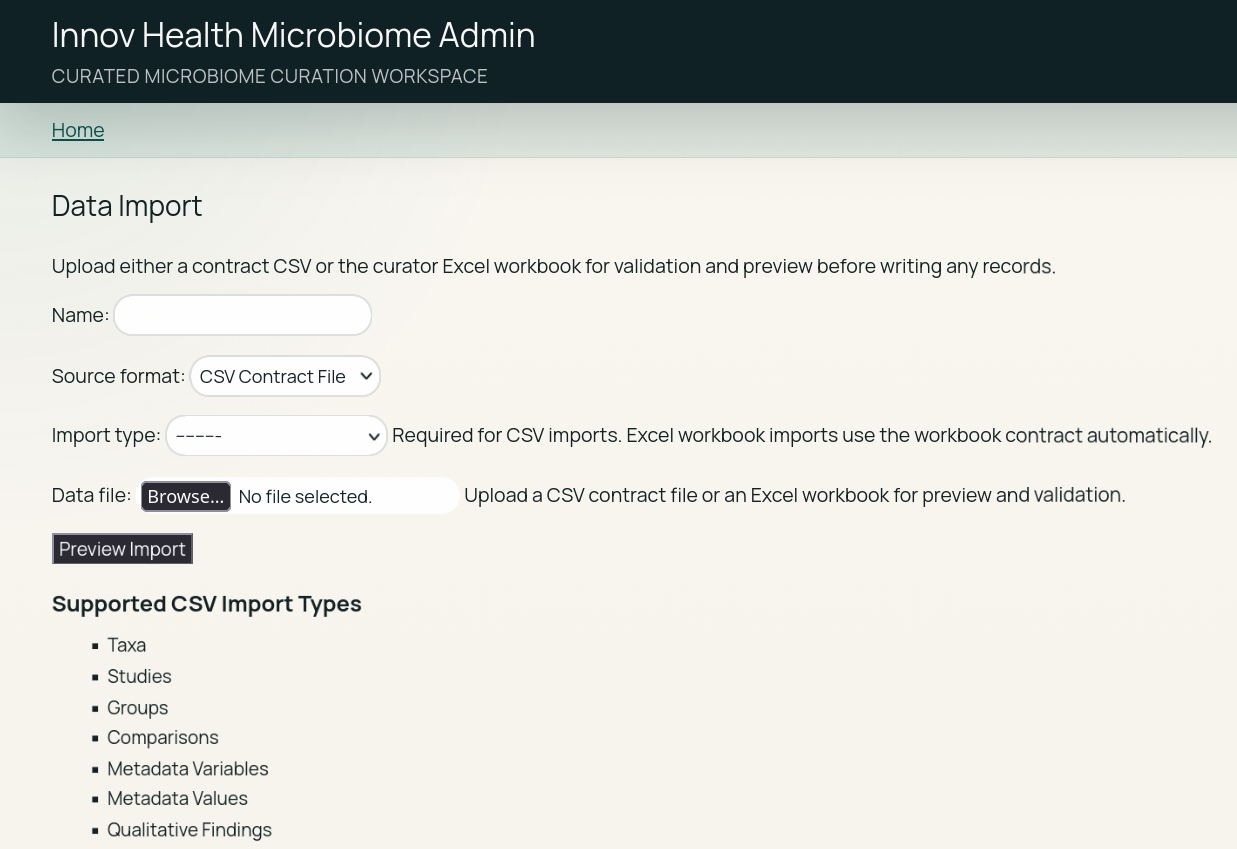
\includegraphics[width=\linewidth]{figures/minddb_admin_import.png}
    \caption{Admin-side workflow for uploading, previewing, and confirming curated data imports before records are written to the database.}
    \label{fig:adminimport}
\end{figure}

\subsection{Graph exploration}

Although the project is not centered on visualization alone, graph-based exploration is a useful extension of the curated database. The current implementation includes an interactive disease--taxon network derived from qualitative findings. Users can apply study and direction filters, constrain the graph to one taxonomic branch, and roll findings up from leaf taxa to higher ranks such as genus or family.

This view is valuable because it gives a compact overview of directional evidence without discarding the underlying database structure. It does not replace the browser; instead, it acts as a second lens over the same curated records.

This is also a useful proof of concept for future work. If qualitative findings can already be organized into a lineage-aware disease--taxon graph, then later extensions such as richer edge summaries, cross-study weighting, or comparative network views become easier to imagine and implement on the same foundation.

\begin{figure}[htbp]
    \centering
    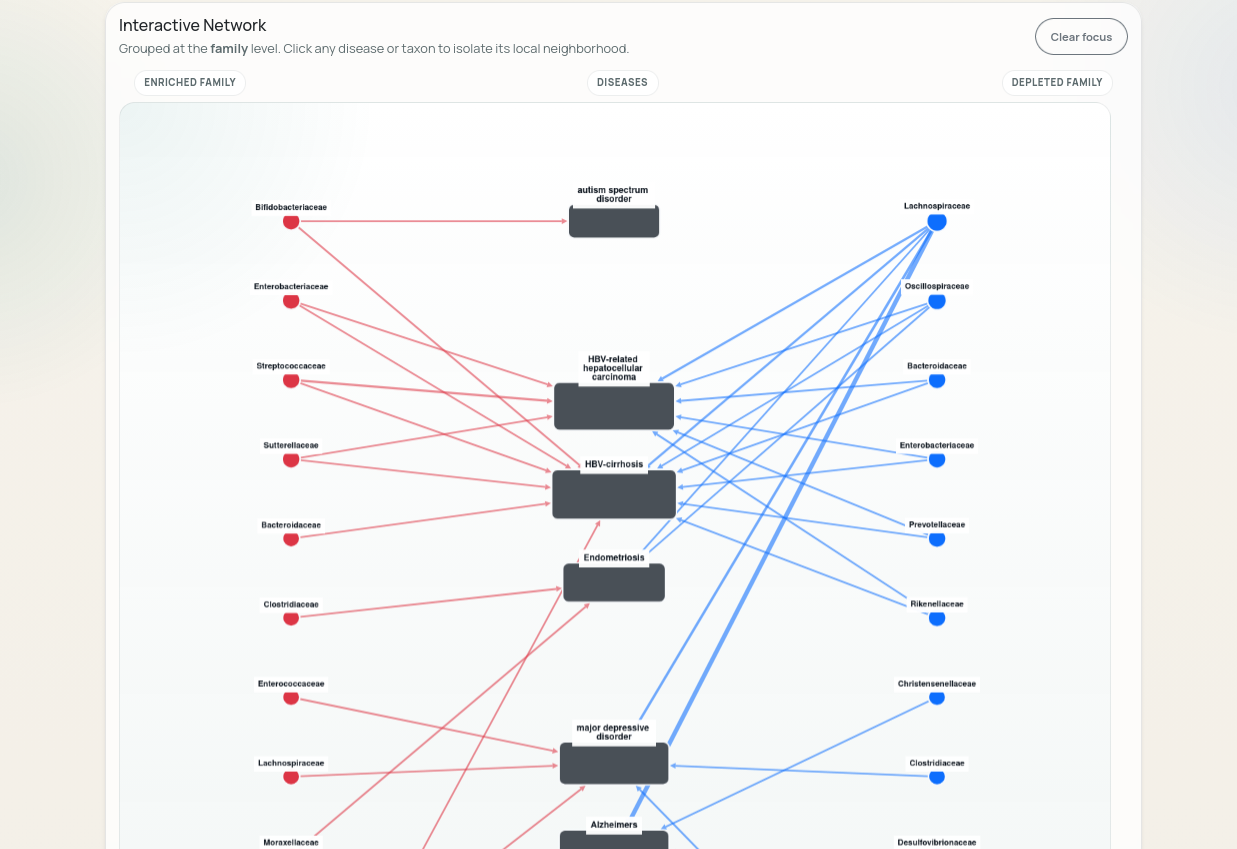
\includegraphics[width=\linewidth]{figures/minddb_graph.png}
    \caption{Interactive graph view showing qualitative disease--taxon relationships derived from curated comparison records.}
    \label{fig:graph}
\end{figure}

\subsection{Taxon Bridge workflow}

Taxon Bridge is most visible during import preview, where incoming names can be resolved, normalized, or flagged for review. This gives curators a chance to inspect organism handling before data are committed. From a usability perspective, this is preferable to either accepting raw names blindly or rejecting ambiguous rows without explanation.

\begin{figure}[htbp]
    \centering
    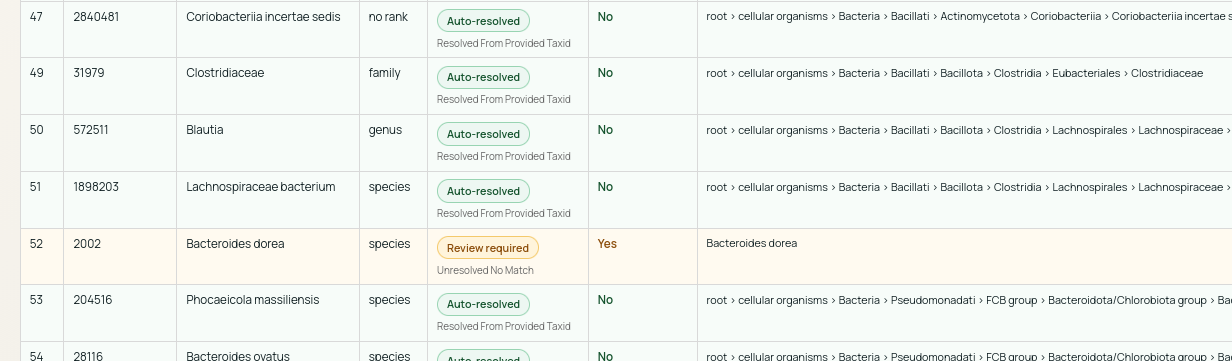
\includegraphics[width=\linewidth]{figures/taxon_bridge_preview.png}
    \caption{Taxon Bridge-assisted preview showing taxonomy-aware resolution before imported findings are committed to the database.}
    \label{fig:taxonbridge}
\end{figure}

\FloatBarrier
